\documentclass{article}
\usepackage{graphicx} % Required for inserting images
\usepackage[T1]{fontenc}
\usepackage{float}
\usepackage{amsfonts}

\title{ON L2}
\author{Maksymilian Neumann}
\date{Listopad 2023}

\begin{document}

\maketitle

\section{Iloczyn skalarny wektorów(małe różnice)}
    \subsection{Wprowadzenie}
    \subsection{Rozwiazanie}
        Rozwiązanie wykonane w języku Julia. Według następujących rozumowań ze wskazanymi zmanami w danych:
        \begin{enumerate}
            \item "w przód" t.j. $\sum^n_{i=1} x_i y_i$
            \item "w tył" t.j. $\sum^1_{i=n} x_i y_i$
            \item "od największego do najmniejszego"
            \item "od najmniejszego do największego"
        \end{enumerate}
    \subsection{Wyniki}
    Uzyskałem następujące wyniki. I porównałem z prawidłową wartością.
    \begin{center}
        \begin{tabular}{|c||c|c|c|}
        \hline
            Źródło & Oryginalny Float32 & Nowy Float32 & Różnica \\
            \hline\hline
            "1" & -0.49994431 & -0.4999443 & 0.0\\
             \hline
             "2" & -0.4543457 & -0.4543457 & 0.0\\
             \hline
             "3" & -0.5 & -0.5 & 0.0\\
             \hline
             "4" & -0.5 & -0.5 & 0.0\\
        \hline
        \end{tabular}
    \end{center}
    \begin{center}
        \begin{tabular}{|c||c|c|c|}
        \hline
            Źródło & Oryginalny Float64 & Nowy Float64 & Różnica \\
            \hline\hline
            "1" & 1.0251881368296672e-10 & -0.004296342739891585 & 0.004296342842410399\\
            \hline
            "2" & -1.5643308870494366e-10 & -0.004296342998713953 & 0.004296342842280865\\
            \hline
            "3"& 0.0 & -0.004296342842280865 & 0.004296342842280865\\
            \hline
            "4"& 0.0 & -0.004296342842280865 & 0.004296342842280865\\
        \hline
        \end{tabular}
    \end{center}
    \subsection{Wnioski}
    We Float64 Wyniki różnią się sporo natomiast we Float32 Wyniki są identyczne ponieważ usunięte liczby znajdowały się na granicy precyzji tej arytmetyki. Wiemy że orygialny iloczyn był równy $-1.0057107*10^{-11}$ z tego możemy obliczyż że nasz zmieniony iloczy będzie równy $-0.004296343192495245$ z tego mnożemy zobaczy że błedy mocno zmalały jak weźmiemy pod uwagę wszytkie nasze sposoby liczenia iloczynu skalarnego. Bardzo minimalna zmiana w danych dała nam duże ulepszenie wyniku co sugeruje nam złe uwarunkowanie początkowego zadania.
\section{Prownanie granic z wykresmi}
    \subsection{Wprowadzenie}
    W tym zadaniu porównujemy wykresy funckji $f(x) = e^xln(1+e^{-x})$ wygenaerowane za pomocą Wolfram Alpha oraz pakietu Plots w języku Julia i porówmujemy je z wartością dokładną z wyniku $\lim_{x\to\infty}f(x)$. 
    \subsection{Rozwiązanie}
    Wykresy zostały wygenerowane przez Wolfram Alpha który oddał nam wykres w przedziale [-18,45] oraz w języku Julia w tym samym przedziale. Następnie obliczyłem granicę.
    \[\lim_{x\to\infty}e^xln(1+e^{-x})=\lim_{x\to\infty}\frac{ln(1+e^{-x})}{e^{-x}}=\lim_{x\to\infty}\frac{-e^{-x}}{(1+e^{-x})*(-e^{-e})}=\lim_{x\to\infty}\frac{1}{1+e^{-x}}=1\]
    \subsection{Wyniki}
    \begin{figure}[H]
        \centering
        \includegraphics[width=0.75\linewidth]{Wolfram plot.png}
        \caption{Wolfram Plot}
        \label{fig:enter-label}
    \end{figure}
    \begin{figure}[H]
        \centering
        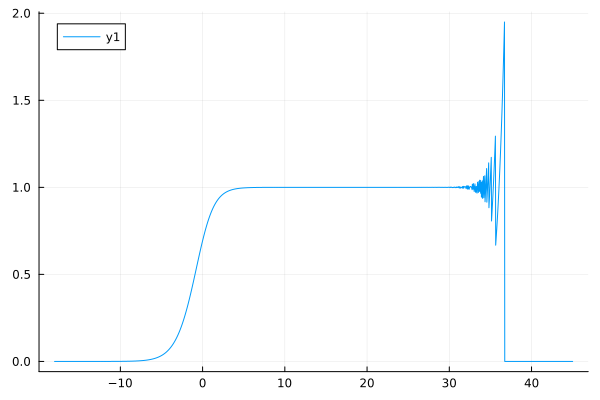
\includegraphics[width=0.75\linewidth]{2.2.png}
        \caption{Julia}
        \label{fig:enter-label}
    \end{figure}
    \subsection{Wnioski}
    Patrząc na naszę wyniki możemy wywnioskować że zadanie jest źle uwarunkowane. Małe błedy wynikające z arytmetyki zmiennoprzecinkowej wowodują gigantyczne błedy dla $x > 30$ nastepnie funkcja spada do 0 i tam się utrzymuje. Dzieje się tak ponieważ dla dużych x: $e^{-x} + 1 \approx 1$ a, $ln(1) = 0$.
\section{Układy równań liniowych z różnymi macierzami}
    \subsection{Wprowadzenie}
    Rozważmy zadanie rozwiązywania układu równań liniowych $Ax=b$ dla danej macierzy współczynników $A \in \mathbb{R}^{n\times n}$ i wekrota $b$. Macież $A$ jest Macieżą Hilberta $H_n$ lub Macierzą losową $R_n$.
    \subsection{Rozwiązanie}
    Wektor $b$ wyznaczamy $b = Ax$ a $x = (1,...,1)^T$ następnie rozwiązujemy to za pomocą eliminacji Gaussa oraz $x=A^{-1}b$. Eksperymenty wykonujemy dla macieży Hilberta z rosnącym $n > 1$ oraz dla $R_n$: $n=5,10,20$ z rosnącym wskaźnikiem uwarunkowania $c=1,10,10^3,10^7,10^12,10^16$ i liczymy błędy względne. Macież Hilberta i oraz Macież losowa wyznaczane są przez dostarczone funkcje.
    \subsection{Wyniki}
    Następujące wykresy przedstawiają średni błąd względny naszych rozwiązań. Eliminacja Gaussa to na wykresach $ge(x)$ a durga to $f(x)$\\
    Dla macierzy Hilberta: 
    \begin{figure}[H]
        \centering
        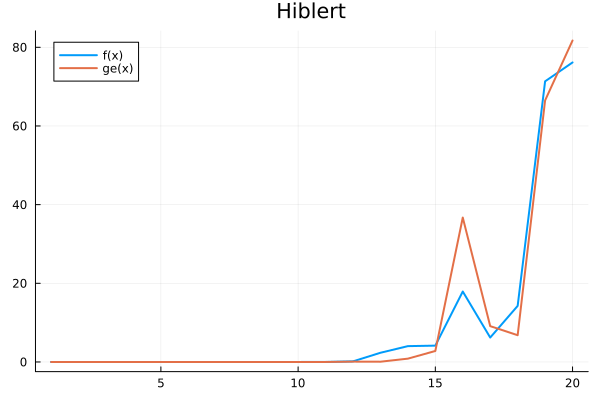
\includegraphics[width=0.75\linewidth]{3.1.png}
        \caption{Hilbert}
        \label{fig:enter-label}
    \end{figure}
    Dla losowych macierzy: 
    \begin{figure}[H]
        \centering
        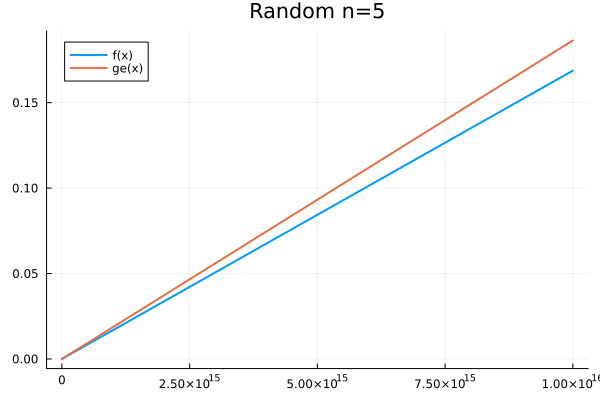
\includegraphics[width=0.75\linewidth]{3.2.png}
        \caption{Hilbert}
        \label{fig:enter-label}
    \end{figure}
    \begin{figure}[H]
        \centering
        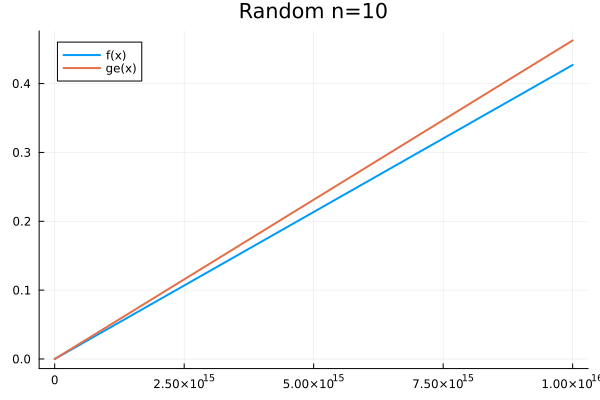
\includegraphics[width=0.75\linewidth]{3.3.png}
        \caption{Hilbert}
        \label{fig:enter-label}
    \end{figure}
    \begin{figure}[H]
        \centering
        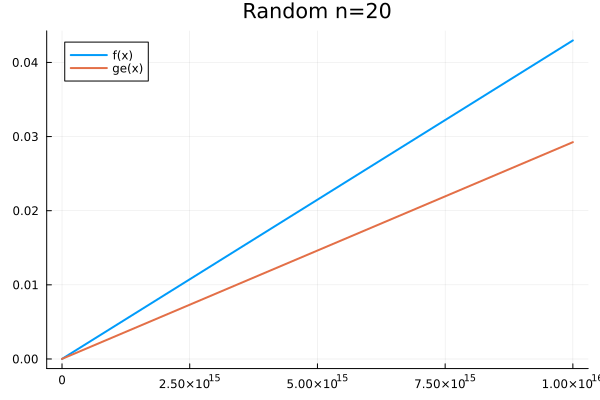
\includegraphics[width=0.75\linewidth]{3.4.png}
        \caption{Hilbert}
        \label{fig:enter-label}
    \end{figure}
    \subsection{Wnioski}
        Żadna z metod nie jest wytaźnie lepsza od drugiej natomiast metoda eliminacji Gaussa wydaje się wychodzić na prowadzenie. Przy obliczeniach przy których kożystaliśmy z macieży Hilberta błędy okazały się być bardzo wysokie ma to związek z wysokim i szybko rosnącym wskaźnikiem uwarunkowania.
        \begin{figure}[H]
            \centering
            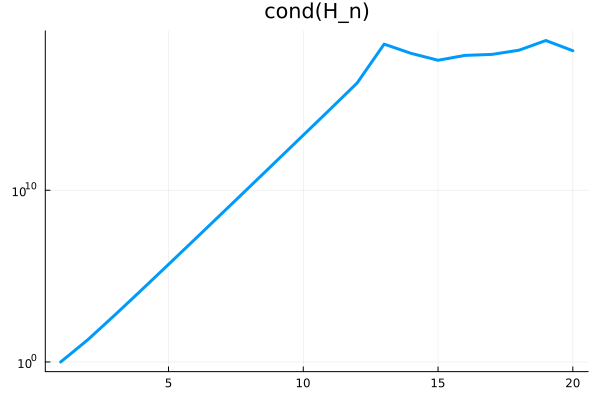
\includegraphics[width=0.75\linewidth]{3.5.png}
            \caption{Uwarunkowanie}
            \label{fig:enter-label}
        \end{figure}
        Natomiast przy losowych macierzach błedy były relatywnie małe a błedy były zbliżone dla macieży o tym samym wskaźniku uwarunkowania a różnych rozmiarów. Możemt w takim razie wnioskować że zadanie z użyciem macieży Hilberta jest źle uwarunkowane.
\section{"Złośliwy Wielomian"}
    \subsection{Wprowadzenie}
    W tym punkcie mamy za zadanie przeanalizować zachowanie "Złośliwego Wielomianu" Wilkinsona sprawdzając obliczone pierwiastki przez bibliotekę Polynomials.
    \subsection{Rozwiązanie}
    Za pomocą biblioteki Polynomials wyznaczamy nasze pierwiastki a następnie obliczamy $|P(z_k)|$ , $|p(z_k)|$ i $|z_k - k|$ gdzie, $P()$ to Wielomian Wilkinsona ze wspołczynników a $p()$ to wielomian z pierwiastków.
    \subsection{Wyniki}
    \begin{figure}[H]
        \centering
        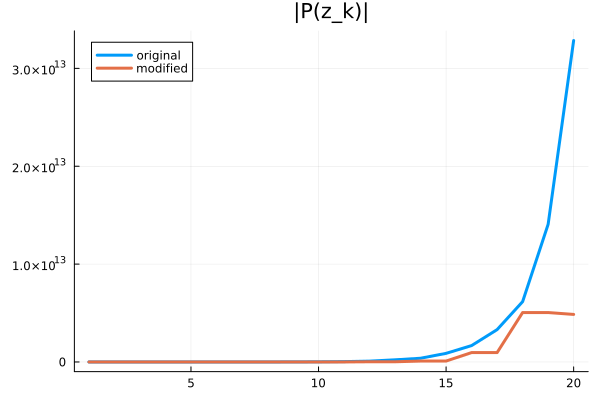
\includegraphics[width=0.75\linewidth]{4.1.png}
        \caption{$|P(z_k)|$}
        \label{fig:enter-label}
    \end{figure}
    \begin{figure}[H]
        \centering
        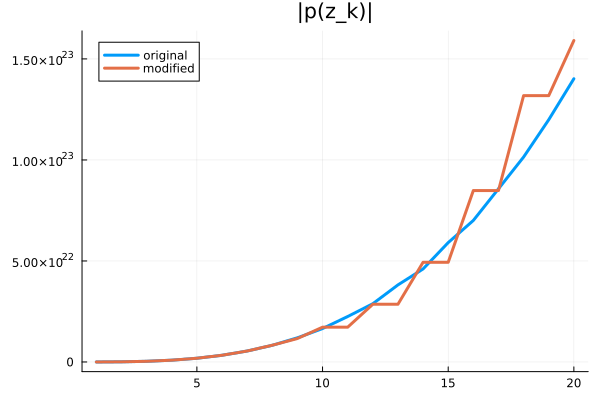
\includegraphics[width=0.75\linewidth]{4.2.png}
        \caption{$|p(z_k)|$}
        \label{fig:enter-label}
    \end{figure}
    \begin{figure}[H]
        \centering
        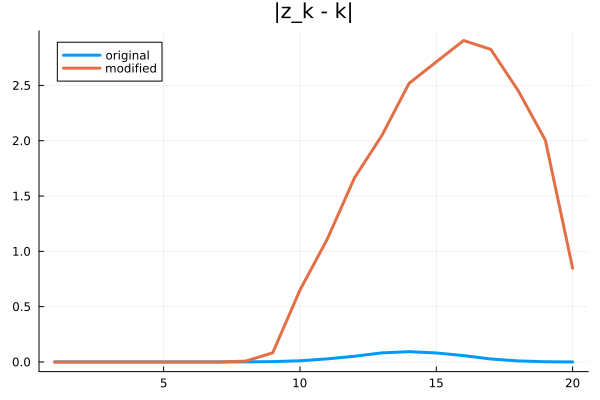
\includegraphics[width=0.75\linewidth]{4.3.png}
        \caption{$|z_k - k|$}
        \label{fig:enter-label}
    \end{figure}
    \subsection{Wnioski}
    Oryginalny wielomian jest relatywnie bliski wartości teoretychych ale prawdziwe pierwiastki nie zerują go więc nie jest aż tak bliski. Tą różnice można zrzucić na niedoskonałości arytmetyki zmiennoprzecinkowej przy przechowywaniu wielomianu w postaci normalnej. Natomiast przy niezwykle małej zmianie naszego wielomianu zaczynają pojawiać się przy pierwiastkach liczby zespolone oraz wartośfi funkcji dla tych pierwiastków są ekstremalnie wysokie. Sugeruje to nam złe uwarunkowanie zadania.
\section{Model Logistyczny, Model Wzrostu Populacji}
    \subsection{Wprowadzenie}
    W tym zadaniu rozważamy równanie rekurencyjne
    $p_{n+1} = p_n + rp_n(1 - p_n)$ dla $n = 0,1,...$ rozważamy czystą implementacje danej funkji oraz zmodyfikowaną implementacje wgdzie przy 10 kroku obcinamy liczby po przeciunku do 3 najbardziej zanczących i je porównujemy. W drugim podpunktcie porównujemy wyniki w arytmetykach Float32 i Float64.
    \subsection{Rozwiązanie}
    Rozwiązanie zostało napisane w Języku Julia.
    \subsection{Wyniki}
\begin{table}[H]
    \centering
    \begin{tabular}{|l|l|l|l|}
    \hline
        \textbf{N} & \textbf{FLOAT32} & \textbf{MODIFIED} & \textbf{FLOAT64} \\ \hline
        \textbf{0} & 0.01 & 0.01 & 0.01 \\ \hline
        \textbf{1} & 0.0397 & 0.0397 & 0.0397 \\ \hline
        \textbf{2} & 0.15407173 & 0.15407173 & 0.15407173000000002 \\ \hline
        \textbf{3} & 0.5450726 & 0.5450726 & 0.5450726260444213 \\ \hline
        \textbf{4} & 1.2889781 & 1.2889781 & 1.2889780011888006 \\ \hline
        \textbf{5} & 0.1715188 & 0.1715188 & 0.17151914210917552 \\ \hline
        \textbf{6} & 0.5978191 & 0.5978191 & 0.5978201201070994 \\ \hline
        \textbf{7} & 1.3191134 & 1.3191134 & 1.3191137924137974 \\ \hline
        \textbf{8} & 0.056273222 & 0.056273222 & 0.056271577646256565 \\ \hline
        \textbf{9} & 0.21559286 & 0.21559286 & 0.21558683923263022 \\ \hline\hline
        \textbf{10} & 0.7229306 & 0.722 & 0.722914301179573 \\ \hline\hline
        \textbf{11} & 1.3238364 & 1.3241479 & 1.3238419441684408 \\ \hline
        \textbf{12} & 0.037716985 & 0.036488414 & 0.03769529725473175 \\ \hline
        \textbf{13} & 0.14660022 & 0.14195944 & 0.14651838271355924 \\ \hline
        \textbf{14} & 0.521926 & 0.50738037 & 0.521670621435246 \\ \hline
        \textbf{15} & 1.2704837 & 1.2572169 & 1.2702617739350768 \\ \hline
        \textbf{16} & 0.2395482 & 0.28708452 & 0.24035217277824272 \\ \hline
        \textbf{17} & 0.7860428 & 0.9010855 & 0.7881011902353041 \\ \hline
        \textbf{18} & 1.2905813 & 1.1684768 & 1.2890943027903075 \\ \hline
        \textbf{19} & 0.16552472 & 0.577893 & 0.17108484670194324 \\ \hline
        \textbf{20} & 0.5799036 & 1.3096911 & 0.5965293124946907 \\ \hline
        \textbf{21} & 1.3107498 & 0.09289217 & 1.3185755879825978 \\ \hline
        \textbf{22} & 0.088804245 & 0.34568182 & 0.058377608259430724 \\ \hline
        \textbf{23} & 0.3315584 & 1.0242395 & 0.22328659759944824 \\ \hline
        \textbf{24} & 0.9964407 & 0.94975823 & 0.7435756763951792 \\ \hline
        \textbf{25} & 1.0070806 & 1.0929108 & 1.315588346001072 \\ \hline
        \textbf{26} & 0.9856885 & 0.7882812 & 0.07003529560277899 \\ \hline
        \textbf{27} & 1.0280086 & 1.2889631 & 0.26542635452061003 \\ \hline
        \textbf{28} & 0.9416294 & 0.17157483 & 0.8503519690601384 \\ \hline
        \textbf{29} & 1.1065198 & 0.59798557 & 1.2321124623871897 \\ \hline
        \textbf{30} & 0.7529209 & 1.3191822 & 0.37414648963928676 \\ \hline
        \textbf{31} & 1.3110139 & 0.05600393 & 1.0766291714289444 \\ \hline
        \textbf{32} & 0.0877831 & 0.21460639 & 0.8291255674004515 \\ \hline
        \textbf{33} & 0.3280148 & 0.7202578 & 1.2541546500504441 \\ \hline
        \textbf{34} & 0.9892781 & 1.3247173 & 0.29790694147232066 \\ \hline
        \textbf{35} & 1.021099 & 0.034241438 & 0.9253821285571046 \\ \hline
        \textbf{36} & 0.95646656 & 0.13344833 & 1.1325322626697856 \\ \hline
        \textbf{37} & 1.0813814 & 0.48036796 & 0.6822410727153098 \\ \hline
        \textbf{38} & 0.81736827 & 1.2292118 & 1.3326056469620293 \\ \hline
        \textbf{39} & 1.2652004 & 0.3839622 & 0.0029091569028512065 \\ \hline
        \textbf{40} & 0.25860548 & 1.093568 & 0.011611238029748606 \\ \hline
    \end{tabular}
\end{table}
\subsection{Wnioski}
Na samym początku wyniki są do siebie bardzo zbliżone natomiast później się coraz bardziej odchylają ma to związek z kumulacją błędu. Kumulacja błedu jest bardzo szybka przez podnoszenie wartości do kwadratu.
\section{Inne Równanie Rekurencyjne}
    \subsection{Wprowadzenie}
    W tym zadaniu rozważamy równanie rekurencyjne
    $p_{n+1} = x^2_n + c$ dla $n = 0,1,...$ gdzie, $c$ jest daną stałą. 
    \subsection{Rozwiązanie}
    Rozwiązanie zostało napisane w Języku Julia. Eksperymenty zostały przeprowadzone dla danych: 
    \begin{enumerate}
        \item $x_0 = 1$, $c = -2$
        \item $x_0 = 2$, $c = -2$
        \item $x_0 = 1.99999999999999$, $c = -2$
        \item $x_0 = 1$, $c = -1$
        \item $x_0 = -1$, $c = -1$
        \item $x_0 = 0.75$, $c = -1$
        \item $x_0 = 0.25$, $c = -1$
    \end{enumerate}
    \subsection{Wyniki}
    \begin{figure}[H]
        \centering
        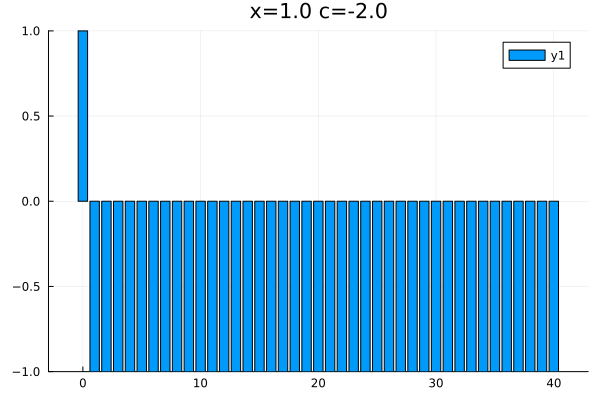
\includegraphics[width=0.75\linewidth]{6 x=1.0 c=-2.0.png}
        \label{fig:enter-label}
    \end{figure}
        \begin{figure}[H]
        \centering
        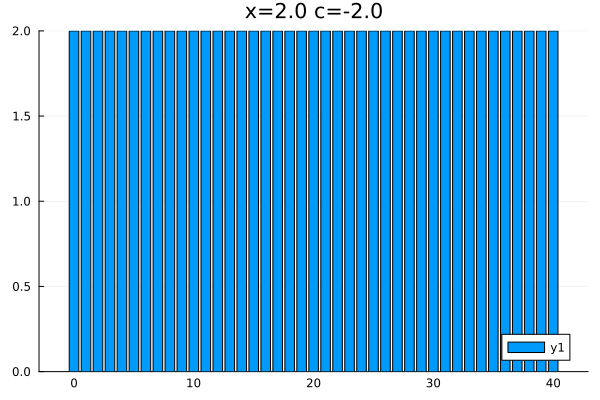
\includegraphics[width=0.75\linewidth]{6 x=2.0 c=-2.0.png}
        \label{fig:enter-label}
    \end{figure}
        \begin{figure}[H][H]
        \centering
        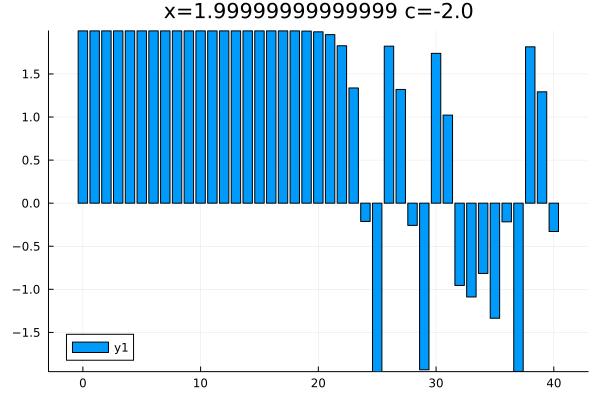
\includegraphics[width=0.75\linewidth]{6 x=1.99999999999999 c=-2.0.png}
        \label{fig:enter-label}
    \end{figure}
        \begin{figure}[H]
        \centering
        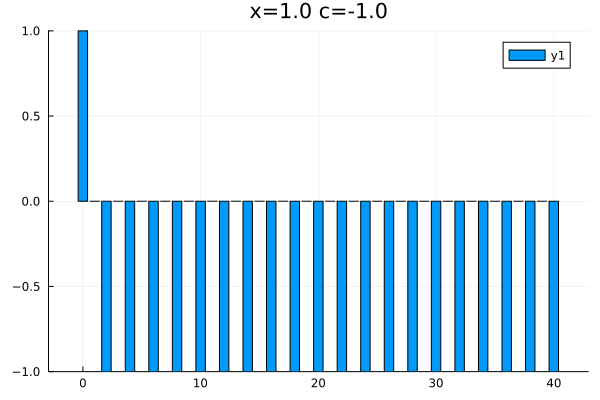
\includegraphics[width=0.75\linewidth]{6 x=1.0 c=-1.0.png}
        \label{fig:enter-label}
    \end{figure}
        \begin{figure}[H]
        \centering
        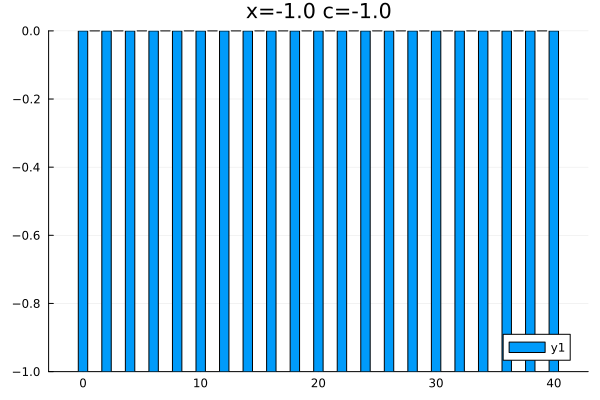
\includegraphics[width=0.75\linewidth]{6 x=-1.0 c=-1.0.png}
        \label{fig:enter-label}
    \end{figure}
        \begin{figure}[H]
        \centering
        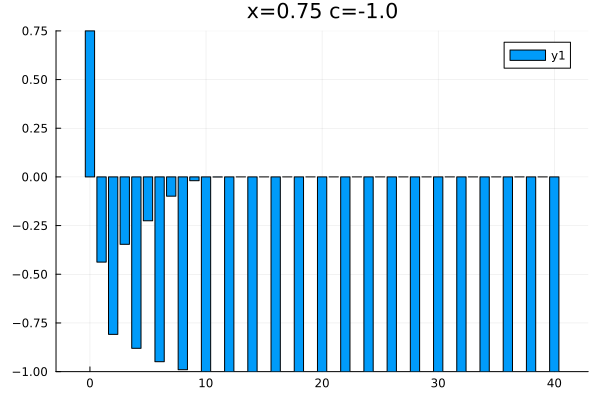
\includegraphics[width=0.75\linewidth]{6 x=0.75 c=-1.0.png}
        \label{fig:enter-label}
    \end{figure}
        \begin{figure}[H]
        \centering
        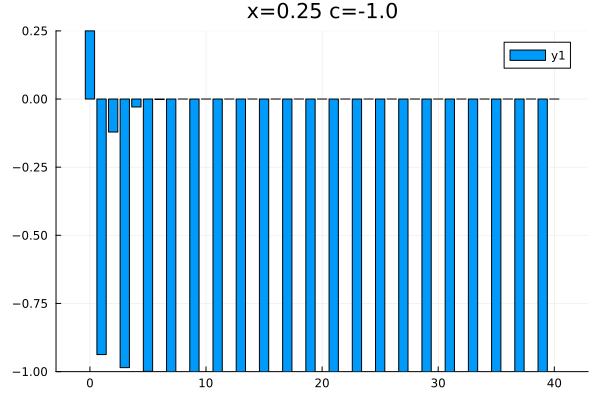
\includegraphics[width=0.75\linewidth]{6 x=0.25 c=-1.0.png}
        \label{fig:enter-label}
    \end{figure}
    \subsection{Wnioski}
\end{document}
